\section{矩形计数}\label{sec:problem85}
\subsection{问题描述}
\begin{tcolorbox}
通过仔细计算,可以发现一个 $3 \times 2$ 的矩形网格包含 18 个矩形:
\vspace{1cm}

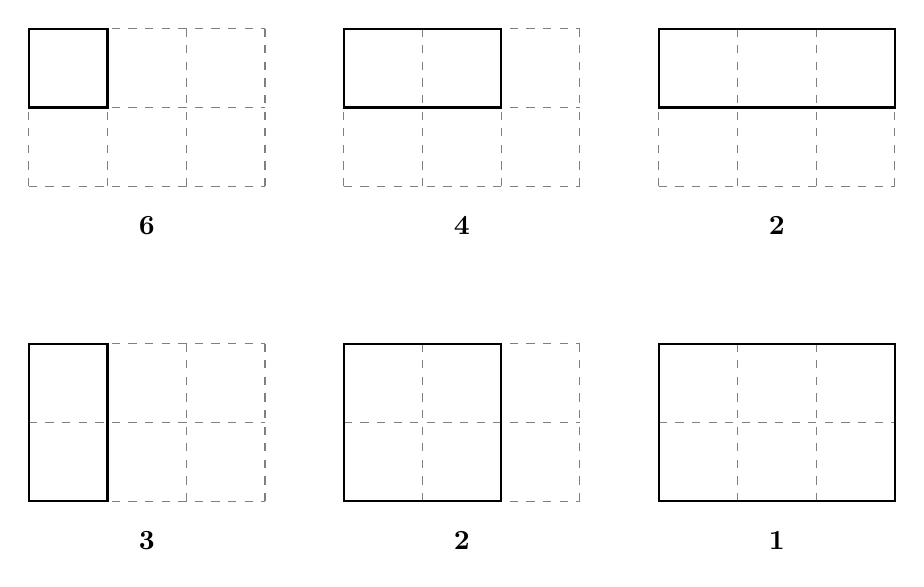
\begin{tikzpicture}

% 第一行
% 左上:6个小矩形
\begin{scope}[xshift=0cm, yshift=-4cm]
    \draw[step=1cm, gray, dashed] (0,0) grid (3,2);
    \draw[thick] (0,1) rectangle (1,2);
    \node at (1.5, -0.5) {\textbf{6}};
\end{scope}

% 中上:4个小矩形
\begin{scope}[xshift=4cm, yshift=-4cm]
    \draw[step=1cm, gray, dashed] (0,0) grid (3,2);
    \draw[thick] (0,1) rectangle (2,2);
    \node at (1.5, -0.5) {\textbf{4}};
\end{scope}

% 右上:2个小矩形
\begin{scope}[xshift=8cm, yshift=-4cm]
    \draw[step=1cm, gray, dashed] (0,0) grid (3,2);
    \draw[thick] (0,1) rectangle (3,2);
    \node at (1.5, -0.5) {\textbf{2}};
\end{scope}

% 第二行
% 左下:3个小矩形
\begin{scope}[xshift=0cm, yshift=-8cm]
    \draw[step=1cm, gray, dashed] (0,0) grid (3,2);
    \draw[thick] (0,0) rectangle (1,2);
    \node at (1.5, -0.5) {\textbf{3}};
\end{scope}

% 中下:2个小矩形
\begin{scope}[xshift=4cm, yshift=-8cm]
    \draw[step=1cm, gray, dashed] (0,0) grid (3,2);
    \draw[thick] (0,0) rectangle (2,2);
    \node at (1.5, -0.5) {\textbf{2}};
\end{scope}

% 右下:1个矩形
\begin{scope}[xshift=8cm, yshift=-8cm]
    \draw[step=1cm, gray, dashed] (0,0) grid (3,2);
    \draw[thick] (0,0) rectangle (3,2);
    \node at (1.5, -0.5) {\textbf{1}};
\end{scope}

\end{tikzpicture}

虽然不存在恰好包含两百万个矩形的矩形网格,但请找出包含的矩形数量最接近两百万的网格的面积。
\end{tcolorbox}

\subsection{算法}
这道题目数矩形可以用以下公式来计算:

假设一个 \( m \times n \)的网格,其中包含的矩形数为
\begin{equation*}
    \dfrac{m(m+1) \cdot n(n+1)}{4}
\end{equation*}

公式可以通过以下方式来推导:
网格有 \( m \)行,则有 \( m + 1 \)条横边,要组成一个矩形,即从 \( m + 1 \)条横边中取 \( 2 \)条边,按照组合公式得共有 \(
m (m + 1) / 2\)种组合,同理竖边有 \( n ( n + 1) / 2 \)种。则可推导出上面的计算公式。

这道题目还要解决离2百万最近的问题,可以依次取$ m=1, 2, \dots $计算出最接近的 $n$。

计算上界的时候要放一些余量来覆盖所有的情况。
\subsection{答案}
2772
